\documentclass{llncs}
\usepackage[utf8]{inputenc}
\usepackage[noend]{algorithmic}
\usepackage{algorithm}
\usepackage{epsfig}
\usepackage{multicol}
\usepackage{multirow}
\usepackage{wrapfig}
\usepackage{subfigure}
\usepackage{url}
\newcommand{\verbatimproperties}{\renewcommand{\baselinestretch}{0.85} \small}

%%%%%%%%%%%%%%%%%%%%%%%%%%%%%%%%%%%%%%%%%%%%%%%%%%%%%%%%%%%%%%%%%%%%%%

\begin{document}

\title{On Extending a Full-Sharing Multithreaded Tabling Design with Batched Scheduling}

\author{Miguel Areias \and Ricardo Rocha}

\institute{CRACS \& INESC TEC and Faculty of Sciences, University of Porto\\
           Rua do Campo Alegre, 1021, 4169-007 Porto, Portugal\\
           \email{\{miguel-areias,ricroc\}@dcc.fc.up.pt}}

\maketitle

%%%%%%%%%%%%%%%%%%%%%%%%%%%%%%%%%%%%%%%%%%%%%%%%%%%%%%%%%%%%%%%%%%%%%%

\begin{abstract}
  Tabling is a technique that overcomes some limitations of
  traditional Prolog systems in dealing with redundant
  sub-computations and recursion. When tabling is combined with
  multithreading, we have the best of both worlds, since we can
  exploit the combination of higher declarative semantics with higher
  procedural control. To support this combination, the Yap Prolog
  system has, at engine level, multiple designs that vary from a
  No-Sharing design, where each thread allocates fully private tables,
  to a Full-Sharing (FS) design, where threads share the complete
  table space. In this work, we propose an extension to the table
  space data structures, which we named \emph{Private Answer Chaining
    (PAC)}, as way to support batched scheduling evaluation with the
  FS design. Batched scheduling is one of the most successful tabling
  scheduling strategies, known to be useful when a tabled logic
  program requires an eager propagation of answers and/or do not
  requires the complete set of answers to be found. Experimental
  results show that PAC is a good first approach, since with it the FS
  design remains quite competitive.\\

\textbf{Keywords:} Logic Programming, Multithreading, Tabling, Scheduling.
\end{abstract}

%%%%%%%%%%%%%%%%%%%%%%%%%%%%%%%%%%%%%%%%%%%%%%%%%%%%%%%%%%%%%%%%%%%%%%

\section{Introduction}

Tabling~\cite{Chen-96} is a technique that overcomes some limitations
of traditional Prolog systems in dealing with redundant
sub-computations and recursion. Tabling consists in storing
intermediate answers for subgoals in a proper data structure, called
the \emph{table space}, so that they can be reused when a repeated
subgoal appears during the resolution process. Tabling has become a
popular and successful technique thanks to the ground-breaking work in
the XSB Prolog system and in particular in the SLG-WAM
engine~\cite{Sagonas-98}, the most successful engine of
XSB. Implementations of tabling are now widely available in systems
like Yap Prolog, B-Prolog, ALS-Prolog, Mercury, Ciao Prolog and more
recently Picat.

Multithreading in Prolog is the ability to concurrently perform
computations, in which each computation runs independently but shares
the program clauses. When multithreading is combined with tabling, we
have the best of both worlds, since we can exploit the combination of
higher procedural control with higher declarative semantics. To the
best of our knowledge, XSB~\cite{Marques-08} and Yap~\cite{Areias-12a}
are the only Prolog systems that support the combination of
multithreading with tabling. In this work, we will focus on Yap's
implementation that follows a SWI-Prolog compatible multithreading
library~\cite{Wielemaker-03}. For tabled evaluation, a thread views
its tables as private but, at the engine level, Yap has three
designs~\cite{Areias-12a}, which vary from a \emph{No-Sharing} (NS)
design, where each thread allocates private tables for each new tabled
subgoal call, to a \emph{Full-Sharing} (FS) design, where threads
share the complete table space.

The decision about the evaluation flow is determined by the
\emph{scheduling strategy}. Different strategies may have a
significant impact on performance, and may lead to a different
ordering of solutions to the query goal. Arguably, the two most
successful tabling scheduling strategies are \emph{local scheduling}
and \emph{batched scheduling}~\cite{Freire-96}. Local scheduling tries
to complete subgoals as soon as possible. When new answers are found,
they are added to the table space and the evaluation fails. Local
scheduling has the advantage of minimizing the size of clusters of
dependent subgoals, however it delays propagation of answers and
requires the complete evaluation of the search space. 

Batched scheduling favors forward execution first, backtracking next,
and consuming answers or completion last. It thus tries to delay the
need to move around the search tree by batching the return of answers
to repeated subgoals. When new answers are found for a particular
tabled subgoal, they are added to the table space and the evaluation
continues. Batched scheduling can be an useful strategy in tabled
logic programs that require an eager propagation of answers and/or do
not require the complete set of answers to be found.

With the FS design, all tables are shared. Thus, since several threads
can be inserting answers in the same table, when an answer already
exists, it is not possible to determine if the answer is new or
repeated for a particular thread without further support. For local
scheduling, this is not a problem since, for repeated and new answers,
local scheduling always fails. The problem is with batched scheduling
that requires that only the repeated answers should fail. Threads have
then to detect, during batched evaluation, whether an answer is new
and must be propagated or whether an answer is repeated and the
evaluation should fail.

In this work, we propose an extension to the table space data
structures, which we named \emph{Private Answer Chaining (PAC)}, as a
way to keep track, per thread and subgoal call, of the answers that
were already found and propagated. We discuss in detail our proposal
for extending the FS design with batched scheduling and we present a
performance analysis comparison between local and batched
scheduling. Experimental results show that, despite the extra PAC data
structures required to support batched scheduling with the FS design,
the execution time of the combination is still quite competitive.

The remainder of the paper is organized as follows. First, we briefly
introduce some background and related work. Then, we describe our PAC
approach and we discuss the most important implementation
details. Finally, we present experimental results and we end by
outlining some conclusions.

%%%%%%%%%%%%%%%%%%%%%%%%%%%%%%%%%%%%%%%%%%%%%%%%%%%%%%%%%%%%%%%%%%%%%%

\section{Background}

The basic idea behind tabling is straightforward: programs are
evaluated by storing answers for tabled subgoals in an appropriate
data space, called the \emph{table space}. Repeated calls\footnote{We
  are considering \emph{variant-based
    tabling}~\cite{RamakrishnanIV-99}. Two tabled subgoals A and B are
  variants if they can be made identical by variable renaming. For
  example, \emph{p(X,1,Y)} and \emph{p(Y,1,Z)} are variants because
  both can be transformed into \emph{p(VAR$_0$,1,VAR$_1$)}.} to tabled
subgoals are not re-evaluated against the program clauses, instead
they are resolved by consuming the answers already stored in their
table entries. During this process, as further new answers are found,
they are stored in their tables and later returned to all repeated
calls.

\begin{wrapfigure}{r}{4.5cm}
\vspace{-\intextsep}
\centering
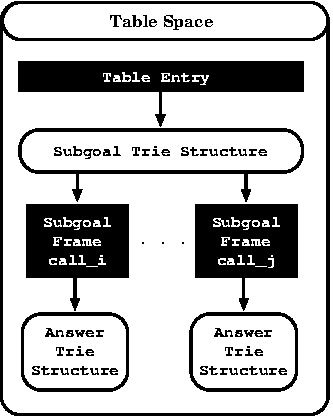
\includegraphics[width=4.5cm]{figures/table_space.pdf}
\caption{Table space organization}
\label{fig_table_space}
\vspace{-\intextsep}
\end{wrapfigure}

Figure~\ref{fig_table_space} shows Yap's table space organization. At
the entry point we have the \emph{table entry} data structure. This
structure is allocated when a tabled predicate is being compiled, so
that a pointer to the table entry can be included in its compiled
code. This guarantees that further calls to the predicate will access
the table space starting from the same point. Below the table entry,
we have the \emph{subgoal trie structure}. Each different tabled
subgoal call to the predicate at hand corresponds to a unique path
through the subgoal trie structure, always starting from the table
entry, passing by several subgoal trie data units, the \emph{subgoal
  trie nodes}, and reaching a leaf data structure, the \emph{subgoal
  frame}. The subgoal frame stores additional information about the
subgoal and acts like an entry point to the \emph{answer trie
  structure}. Each unique path through the answer trie data units, the
\emph{answer trie nodes}, corresponds to a different answer to the
entry subgoal.

%%%%%%%%%%%%%%%%%%%%%%%%%%%%%%%%%%%%%%%%%%%%%%%%%%%%%%%%%%%%%%%%%%%%%%

\subsection{Yap's Multithreaded Tabling Support}

In Yap, a thread views its tables as private but, at the engine level,
it implements three designs for concurrent tabling support that vary
from a \emph{No-Sharing} (NS) design, where each thread allocates
fully private tables, to a \emph{Full-Sharing} (FS) design, where
threads share the complete table
space. Figure~\ref{fig_yap_mt_support} shows Yap's multithreaded table
space organization for the NS and FS designs, where an interface layer
abstracts the design being used at the engine level. The figure
illustrates the main differences between the two designs for a
situation where several threads are evaluating the same tabled subgoal
call $call\_i$.

\begin{figure}[!ht]
%\vspace{-\intextsep}
\centering
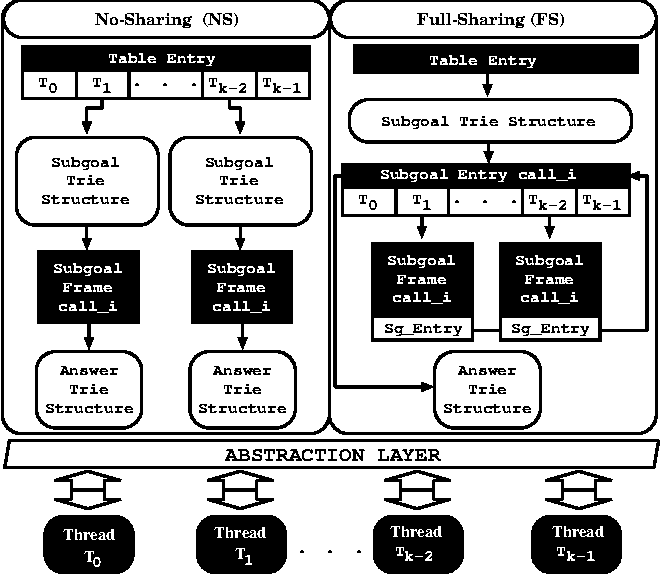
\includegraphics[width=9.5cm]{figures/yap_mt.pdf}
\caption{Yap's multithreaded table space organization for the NS and FS designs}
\label{fig_yap_mt_support}
\vspace{-\bigskipamount}
\end{figure}

When using the NS design, one can observe that the table entry data
structure still stores the common information for the predicate (such
as the arity or the scheduling strategy), and then each thread $t$ has
its own cell $T_t$ inside a \emph{bucket array} which points to the
private data structures.

When using the FS design, the subgoal and answer trie structures and
part of the subgoal frame information (the \emph{subgoal entry} data
structure in Fig.~\ref{fig_yap_mt_support}) are shared among all
threads. The previous subgoal frame data structure was split in two:
the \emph{subgoal entry} stores common information for the subgoal
call (such as the pointer to the shared answer trie structure); the
remaining information is kept private to each thread in the
\emph{subgoal frame} data structure.

%%%%%%%%%%%%%%%%%%%%%%%%%%%%%%%%%%%%%%%%%%%%%%%%%%%%%%%%%%%%%%%%%%%%%%

\subsection{Scheduling Strategies}

Local scheduling evaluates a tabled logic program in a breath-first
manner. It favors backtracking first with completion instead of
forward execution, leaving the consumption of answers for last. Local
scheduling only allows a \emph{Cluster of Dependent Subgoals} (CDS) to
return answers after a fix-point has been reached~\cite{Freire-96}. In
other words, local scheduling tries to keep a CDS as minimal as
possible, thus creating less complex dependencies between subgoals,
which causes a sooner completion of subgoals.

On the other hand, batched scheduling evaluates a tabled logic program
in a depth-first manner. It favors the forward execution first instead
of backtracking, leaving the consumption of answers and completion for
last. It thus tries to delay the need to move around the search tree
by batching the return of answers. When new answers are found for a
particular tabled subgoal, they are added to the table space and the
execution continues. For some situations, this results in creating
dependencies to older subgoals, therefore enlarging the current CDS
and delaying the fix-point that guarantees that all dependent subgoals
in a CDS are completely evaluated~\cite{Sagonas-98}. Batched
scheduling can be an useful strategy in tabled logic programs that
require an eager propagation of answers and/or do not require the
complete set of answers to be found.

%%%%%%%%%%%%%%%%%%%%%%%%%%%%%%%%%%%%%%%%%%%%%%%%%%%%%%%%%%%%%%%%%%%%%%

\section{Extending Full-Sharing with Batched Scheduling}

\begin{wrapfigure}{r}{6.5cm}
\vspace{-\intextsep}
\centering
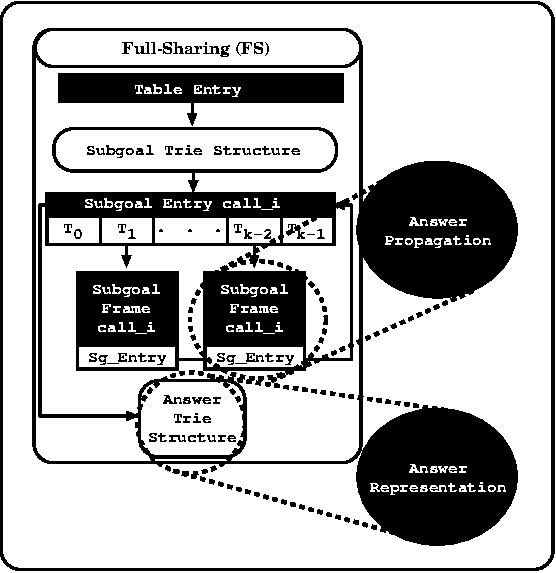
\includegraphics[width=6.4cm]{figures/pac_overview.pdf}
\caption{PAC overview}
\label{fig_pac_overview}
\vspace{-\intextsep}
\end{wrapfigure}

In this section, we describe our proposal to support the combination
of batched scheduling with the FS design. In the original FS design,
answer propagation and answer representation are both stored in the
answer trie data structure, thus threads are unable to distinguish
whether they have or not have propagated an answer already stored in
the table space. To solve that, we propose an extension to the table
space data structures, which we named \emph{Private Answer Chaining}
(PAC), as a way to keep track, per thread and subgoal call, of the
answers that were already found and propagated to the thread's
repeated calls. Figure~\ref{fig_pac_overview} illustrates PAC's key
idea. In a nutshell, PAC splits answer propagation from answer
representation, and allows the first to be privately stored in the
subgoal frame data structure of each thread, and the second to be kept
publicly shared among threads in the answer trie data structure.

%%%%%%%%%%%%%%%%%%%%%%%%%%%%%%%%%%%%%%%%%%%%%%%%%%%%%%%%%%%%%%%%%%%%%%

\subsection{Our Approach}

The PAC procedure works at the subgoal frame level. The key idea is to
extend subgoal frames with an auxiliary private chaining of answers
for each subgoal call, in order to keep track of the answers already
found for the call. Later, if a thread completes a subgoal's
evaluation, i.e, if the subgoal's table is marked as complete, its PAC
is made public, so that from that point on all threads can use that
chain in complete (only reading) mode. Figure~\ref{fig_pac_details}
illustrates the new data structures involved in the implementation of
our PAC's proposal for a situation where different threads are
evaluating the same tabled subgoal call $call\_i$.

\begin{figure}[!ht]
%\vspace{-\intextsep}
\centering
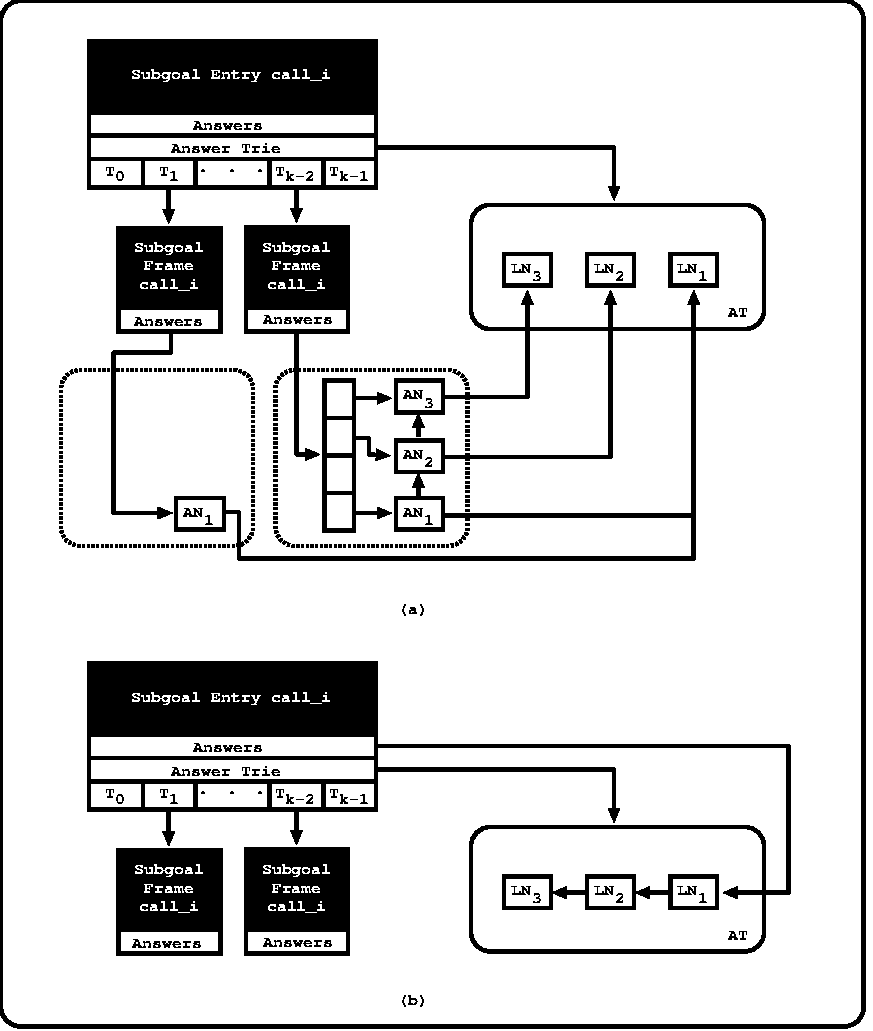
\includegraphics[width=10.5cm]{figures/pac.pdf}
\caption{PAC's data structures for (a) private and (b) public
  chaining}
\label{fig_pac_details}
\vspace{-\bigskipamount}
\end{figure}

Figure~\ref{fig_pac_details}(a) shows then a situation where two
threads, $T_1$ and $T_{k-2}$, are sharing the same subgoal entry for a
call $call\_i$ still under evaluation, i.e., still not yet
completed. The current state of the evaluation shows an answer trie
with 3 answers found for $call\_i$. For the sake of simplicity, we are
omitting the internal answer trie nodes and we are only showing the
leaf nodes $LN_1$, $LN_2$ and $LN_3$ of each answer.

With PAC support, the leaf nodes are not chained in the answer trie
data structure, as usual. Now, the chaining process is done privately,
and for that, we use the subgoal frame structure of each thread. On
the subgoal frame structure we added a new field, called
\emph{Answers}, to store the answers found within the execution of the
thread. In order to minimize PAC's impact, each answer node in the
private chaining has only two fields: (i) an entry pointer, which
points to the corresponding leaf node in the answer trie data
structure; and (ii) a next pointer to chain the nodes in the private
chaining. To maintain good performance, when the number of answer
nodes exceeds a certain threshold, we use a hash trie mechanism design
similar to the one presented in~\cite{Areias-ijpp15}, but without
concurrency support, since this mechanism is private to each thread.

PAC's data structures in Fig.~\ref{fig_pac_details}(a) represent then
two different situations. Thread $T_1$ has only found one answer and
it is using a direct answer chaining to access the leaf node
$LN_1$. Thread $T_{k-2}$ was already found three answers for $call\_i$
and it is using the hash trie mechanism within its private
chaining. In the hash trie mechanism, the answer nodes are still
chained between themselves, thus that repeated calls belonging to
thread $T_{k-2}$ can consume the answers as in the original mechanism.

Figure~\ref{fig_pac_details}(b) shows the state of the subgoal call
after completion. When a thread $T$ completes a subgoal call, it frees
its private consumer structures, but before doing that, it checks
whether another thread as already marked the subgoal as completed. If
no other thread has done that, then thread $T$ not only follows its
private chaining mechanism, as it would for freeing its private nodes,
but also follows the pointers to the answer trie leaf nodes in order
to create a chain inside the answer trie. Since this procedure is done
inside a critical region, no more than one thread can be doing this
chaining process. Thus, in Fig.~\ref{fig_pac_details}(b), we are
showing the situation where the subgoal call $call\_i$ is completed
and both threads $T_1$ and $T_{k-2}$ have already chained the leaf
nodes inside the answer trie and removed their private chaining
structures.

%%%%%%%%%%%%%%%%%%%%%%%%%%%%%%%%%%%%%%%%%%%%%%%%%%%%%%%%%%%%%%%%%%%%%%

\subsection{Implementations Details}

The major difference between local and batched scheduling, at the
engine level, is in the \emph{tabled new answer} operation, where we
decide what to do when a new answer is found during the
evaluation. This operation checks whether a newly found answer is
already in the corresponding answer trie structure and, if not,
inserts it. For local scheduling, it then fails and, for batched
scheduling, it proceeds with forward
execution. Algorithm~\ref{alg_table_new_answer_batched} shows how we
have extended this operation to support the FS design with batched
scheduling.

\vspace{-\bigskipamount}
\begin{algorithm} [!ht]
\caption{tabled\_new\_answer(answer ANS, subgoal frame SF)}
\begin{algorithmic}[1]
  \STATE $leaf \gets check\_insert\_answer\_trie(ANS, SF)$
  \STATE $chain \gets check\_insert\_consumer\_chain(leaf, SF)$
  \IF {$is\_answer\_marked\_as\_found(chain)$}
    \RETURN $failure$
  \ELSE                                        [the answer is new]
    \STATE $mark\_answer\_as\_found(chain)$
    \IF {$local\_scheduling\_mode(SF)$}
      \RETURN $failure$
    \ELSE                                [batched scheduling mode]
      \RETURN $proceed$
    \ENDIF
  \ENDIF  
\end{algorithmic}
\label{alg_table_new_answer_batched}
\end{algorithm}
\vspace{-\bigskipamount}

The algorithm receives two arguments: the newly found answer during
the evaluation (\emph{ANS}) and the subgoal frame which corresponds to
the call at hand (\emph{SF}). The algorithm begins by
checking/inserting the given \emph{ANS} into the answer trie
structure, which will return the leaf node for the path representing
\emph{ANS} (line 1). Then, it checks/inserts the given \emph{leaf}
node into the private chaining for the current thread, which will
return the corresponding answer chain node (line 2). Next in line 3,
it tests whether the answer chain node already existed in the chain,
i.e., if it was inserted or not by the current check/insert operation
in order to return failure (line 4), or it proceeds with marking the
answer \emph{ANS} has found (line 6). At the end (lines 7 to 10), it
returns failure, if local scheduling is active (line 8), otherwise,
batched scheduling is active, and it proceeds by propagating the
answer \emph{ANS} to the current execution environment (line 10).

%%%%%%%%%%%%%%%%%%%%%%%%%%%%%%%%%%%%%%%%%%%%%%%%%%%%%%%%%%%%%%%%%%%%%%

\section{Performance Analysis}

We now present experimental results about the usage of PAC in the FS
design with batched scheduling. Since without PAC the FS design would
not be able to be used with batched scheduling, to put PAC's results
in perspective, we will be showing also the results for local
scheduling and for the NS design. The environment for our experiments
was a machine with 32-Core AMD Opteron (TM) Processor 6274 (2 sockets
with 16 cores each) with 32GB of main memory, running the Linux kernel
3.16.7-200.fc20.x86\_64 with Yap Prolog 6.3. For the experiments, we
used the \emph{TabMalloc} memory allocator~\cite{Areias-12b} and the
set of benchmarks described in~\cite{Areias-12b}. These benchmarks
create \emph{worst case scenarios}, where we are able to show the
lowest bounds of performance that each design might achieve when
applied/used in other real world applications/programs.

Table~\ref{tab_batched_overhead} shows the overhead ratios, when
comparing against the NS design with 1 thread (running with local
scheduling and without TabMalloc), for the NS and FS designs with 1,
8, 16, 24 and 32 threads, using local scheduling (column \emph{Local})
and batched scheduling (column \emph{Batched}) strategies with
TabMalloc. In order to give a fair weight to each benchmark, the
overhead ratio is calculated as follows. We begin by running 10 times
each benchmark $B$ for each design $D$ with $T$ threads. Then, we
calculate the average of those ten runs and use that value ($D_{BT}$)
to put it in perspective against the base time, which is the average
of 10 runs of the NS design with 1 thread ($NS_{B1}$). For that, we
use the following formula for the overhead $O_{DBT} = D_{BT} /
NS_{B1}$. After calculating all the overheads $O_{DBT}$ for a certain
design $D$ and number of threads $T$ corresponding to the several
benchmarks $B$, we calculate the respective minimum, average, maximum
and standard deviation overhead ratios (rows \emph{Min}, \emph{Avg},
\emph{Max} and \emph{StD} in Table~\ref{tab_batched_overhead}).

\setlength{\tabcolsep}{12pt}
\begin{table}[!ht]
\centering
\caption{Overhead ratios, when compared with the NS design with $1$
  thread (running with local scheduling and without TabMalloc) for the
  NS and FS designs (with TabMalloc) when running 1, 8, 16, 24 and 32
  threads with local and batched scheduling (best ratios by row and
  design for the Minimum, Average and Maximum are in bold)}
\begin{tabular}{ll||cc|cc}
\multicolumn{2}{c||}{\multirow{2}{*}{\bf Threads}} &
\multicolumn{2}{c|}{\multirow{1}{*}{\bf NS}} &
\multicolumn{2}{|c}{\multirow{1}{*}{\bf FS}}\\ \cline{3-6}
& 
& \multicolumn{1}{c}{\bf Local}
& \multicolumn{1}{c}{\bf Batched}
& \multicolumn{1}{|c}{\bf Local}
& \multicolumn{1}{c}{\bf Batched}\\
\hline\hline
\multirow{4}{*}{\bf 1}
& {\bf Min }& {\bf 0.53}& 0.55& 1.01& {\bf 0.95}\\
& {\bf Avg }& {\bf 0.78}& 0.82& {\bf 1.30}& 1.46\\
& {\bf Max }& 1.06& {\bf 1.05}& {\bf 1.76}& 2.33\\
& {\bf StD }& 0.15& 0.14& 0.22& 0.44\\
\hline
\multirow{4}{*}{\bf 8}
& {\bf Min }& 0.66& {\bf 0.63}& 1.16&{\bf  0.99}\\
& {\bf Avg }& {\bf 0.85}& 0.88& {\bf 1.88}& 1.95\\
& {\bf Max }& {\bf 1.12}& 1.14& {\bf 2.82}& 3.49\\
& {\bf StD }& 0.13& 0.14& 0.60& 0.79\\
\hline
\multirow{4}{*}{\bf 16}
& {\bf Min }& 0.85& {\bf 0.75}& 1.17& {\bf 1.06}\\
& {\bf Avg }& {\bf 0.98}& 1.00& {\bf 1.97}& 2.08\\
& {\bf Max }& {\bf 1.16}& 1.31& {\bf 3.14}& 3.69\\
& {\bf StD }& 0.09& 0.17& 0.65& 0.83\\
\hline
\multirow{4}{*}{\bf 24}
& {\bf Min }& {\bf 0.91}& 0.93& 1.16& {\bf 1.09}\\
& {\bf Avg }& {\bf 1.15}& 1.16& {\bf 2.06}& 2.19\\
& {\bf Max }& 1.72& {\bf 1.60}& {\bf 3.49}& 4.08\\
& {\bf StD }& 0.20& 0.21& 0.70& 0.91\\
\hline
\multirow{4}{*}{\bf 32}
& {\bf Min }& 1.05& {\bf 1.04}& 1.33& {\bf 1.26}\\
& {\bf Avg }& 1.51& {\bf 1.49}& {\bf 2.24}& 2.41\\
& {\bf Max }& {\bf 2.52}& 2.63& {\bf 3.71}& 4.51\\
& {\bf StD }& 0.45& 0.45& 0.74& 1.02\\
\end{tabular}
\label{tab_batched_overhead}
\end{table}

By observing Table~\ref{tab_batched_overhead}, we can see that batched
scheduling always achieves the best minimum overhead ratio in the FS
design but, for the average and maximum overhead ratios, the best
strategy is always local scheduling. For the average and maximum
overhead ratios, the difference between local and batched scheduling
in the FS design is slightly higher than in the NS design, which can
be read as an indication of the overhead that PAC introduces into the
FS design. Recall that whenever an answer is found during the
evaluation, PAC requires that threads traverse their private consumer
data structures to check if the answer was already found (and propagated).

As we increase the number of threads, for the NS design, both
scheduling strategies show very close minimum, average and maximum
overhead ratios. For the FS design, the differences are slightly
higher. However, for the average overhead ratio, the results between
both strategies are quite close, with batched scheduling being around
10\% slower than local scheduling for the FS design. In summary, our
experimental results show that, on average, the PAC strategy does not
seem to have a big impact in the performance, however it still leaves
room for further improvements, since the difference between local and
batched scheduling is higher in the FS design than in the NS design.

%%%%%%%%%%%%%%%%%%%%%%%%%%%%%%%%%%%%%%%%%%%%%%%%%%%%%%%%%%%%%%%%%%%%%%

\section{Conclusions and Further Work}

Local and batched scheduling are arguably two of the most well-known
tabling scheduling strategies. The major difference between both is
that local scheduling propagates answers only after all answers are
found, while batched scheduling propagates answers immediately after
they are found. Batched scheduling is a useful strategy in tabled
logic programs that require an eager propagation of answers and/or do
not require the complete set of answers to be found. In this work, we
have presented the PAC strategy, which is a simple and novel approach
for combining the FS design with batched scheduling. PAC splits answer
representation from answer propagation, and allows the first to be
publicly shared among threads while the second to be private to each
thread.

Experimental results in worst-case scenarios showed that, on average,
the PAC strategy does not seem to have a big impact in the
performance, however it still leaves room for further improvements
specially in the extra structures required to control the propagated
answers. Further work will include the usage of time-stamped tries to
minimize the search for the propagated answers and new real-world
problems that will allow us to improve and consolidate our framework.

%%%%%%%%%%%%%%%%%%%%%%%%%%%%%%%%%%%%%%%%%%%%%%%%%%%%%%%%%%%%%%%%%%%%%%

\section*{Acknowledgments}

This work is partially funded by project SIBILA
(NORTE-07-0124-FEDER-000059) under the North Portugal Regional
Operational Programme (ON.2 – O Novo Norte) and under the National
Strategic Reference Framework (NSRF), through the European Regional
Development Fund (ERDF) and, by national funds, through the Portuguese
Foundation for Science and Technology (FCT).

%%%%%%%%%%%%%%%%%%%%%%%%%%%%%%%%%%%%%%%%%%%%%%%%%%%%%%%%%%%%%%%%%%%%%%

\bibliographystyle{splncs}
\bibliography{references}

%%%%%%%%%%%%%%%%%%%%%%%%%%%%%%%%%%%%%%%%%%%%%%%%%%%%%%%%%%%%%%%%%%%%%%

\end{document}
